%% For double-blind review submission
\documentclass[sigplan,10pt]{acmart}\settopmatter{printfolios=true}
%% For single-blind review submission
%\documentclass[sigplan,10pt,review]{acmart}\settopmatter{printfolios=true}
%% For final camera-ready submission
%\documentclass[sigplan,10pt]{acmart}\settopmatter{}

%% Note: Authors migrating a paper from traditional SIGPLAN
%% proceedings format to PACMPL format should change 'sigplan,10pt' to
%% 'acmlarge'.


%% Some recommended packages.
\usepackage{booktabs}   %% For formal tables:
                        %% http://ctan.org/pkg/booktabs
\usepackage{subcaption} %% For complex figures with subfigures/subcaptions
                        %% http://ctan.org/pkg/subcaption


\makeatletter\if@ACM@journal\makeatother
%% Journal information (used by PACMPL format)
%% Supplied to authors by publisher for camera-ready submission
\acmJournal{PACMPL}
\acmVolume{1}
\acmNumber{1}
\acmArticle{1}
\acmYear{2017}
\acmMonth{1}
\acmDOI{10.1145/nnnnnnn.nnnnnnn}
\startPage{1}
\else\makeatother
%% Conference information (used by SIGPLAN proceedings format)
%% Supplied to authors by publisher for camera-ready submission
%\acmConference[PL'17]{ACM SIGPLAN Conference on Programming Languages}{January 01--03, 2017}{New York, NY, USA}
%\acmYear{2017}
%\acmISBN{978-x-xxxx-xxxx-x/YY/MM}
%\acmDOI{10.1145/nnnnnnn.nnnnnnn}
%\startPage{1}
%\fi


%% Copyright information
%% Supplied to authors (based on authors' rights management selection;
%% see authors.acm.org) by publisher for camera-ready submission
\setcopyright{none}             %% For review submission
%\setcopyright{acmcopyright}
%\setcopyright{acmlicensed}
%\setcopyright{rightsretained}
%\copyrightyear{2017}           %% If different from \acmYear


%% Bibliography style
\bibliographystyle{ACM-Reference-Format}
%% Citation style
%% Note: author/year citations are required for papers published as an
%% issue of PACMPL.
%\citestyle{acmauthoryear}  %% For author/year citations
%\citestyle{acmnumeric}     %% For numeric citations
%\setcitestyle{nosort}      %% With 'acmnumeric', to disable automatic
                            %% sorting of references within a single citation;
                            %% e.g., \cite{Smith99,Carpenter05,Baker12}
                            %% rendered as [14,5,2] rather than [2,5,14].
%\setcitesyle{nocompress}   %% With 'acmnumeric', to disable automatic
                            %% compression of sequential references within a
                            %% single citation;
                            %% e.g., \cite{Baker12,Baker14,Baker16}
                            %% rendered as [2,3,4] rather than [2-4].



\begin{document}

%% Title information
\title[Human Constraint Layout]         %% [Short Title] is optional;
{High-Level, User-Defined \\Constraints for Graph Layout}         
                                        %% when present, will be used in
                                        %% header instead of Full Title.
%\titlenote{with title note}             %% \titlenote is optional;
                                        %% can be repeated if necessary;
                                        %% contents suppressed with 'anonymous'
%\subtitle{Subtitle}                     %% \subtitle is optional
%\subtitlenote{with subtitle note}       %% \subtitlenote is optional;
                                        %% can be repeated if necessary;
                                        %% contents suppressed with 'anonymous'


%% Author information
%% Contents and number of authors suppressed with 'anonymous'.
%% Each author should be introduced by \author, followed by
%% \authornote (optional), \orcid (optional), \affiliation, and
%% \email.
%% An author may have multiple affiliations and/or emails; repeat the
%% appropriate command.
%% Many elements are not rendered, but should be provided for metadata
%% extraction tools.

%% Author with single affiliation.
\author{Jane Hoffswell}
%\authornote{with author1 note}          %% \authornote is optional;
                                        %% can be repeated if necessary
%\orcid{nnnn-nnnn-nnnn-nnnn}             %% \orcid is optional
\affiliation{
  %\position{Position1}
  %% \department is recommended
  \department{Paul G. Allen School of Computer Science \& Engineering}
  \institution{University of Washington}%% \institution is required
  %\streetaddress{Street1 Address1}
  \city{Seattle}
  \state{WA}
  \postcode{98195}
  \country{United States}
}
%\email{first1.last1@inst1.edu}          %% \email is recommended

%% Author with two affiliations and emails.
% \author{First2 Last2}
% \authornote{with author2 note}          %% \authornote is optional;
%                                         %% can be repeated if necessary
% \orcid{nnnn-nnnn-nnnn-nnnn}             %% \orcid is optional
% \affiliation{
%   \position{Position2a}
%   \department{Department2a}             %% \department is recommended
%   \institution{Institution2a}           %% \institution is required
%   \streetaddress{Street2a Address2a}
%   \city{City2a}
%   \state{State2a}
%   \postcode{Post-Code2a}
%   \country{Country2a}
% }
% \email{first2.last2@inst2a.com}         %% \email is recommended
% \affiliation{
%   \position{Position2b}
%   \department{Department2b}             %% \department is recommended
%   \institution{Institution2b}           %% \institution is required
%   \streetaddress{Street3b Address2b}
%   \city{City2b}
%   \state{State2b}
%   \postcode{Post-Code2b}
%   \country{Country2b}
% }
% \email{first2.last2@inst2b.org}         %% \email is recommended


%% Paper note
%% The \thanks command may be used to create a "paper note" ---
%% similar to a title note or an author note, but not explicitly
%% associated with a particular element.  It will appear immediately
%% above the permission/copyright statement.
% \thanks{with paper note}                %% \thanks is optional
                                        %% can be repeated if necesary
                                        %% contents suppressed with 'anonymous'


%% Abstract
%% Note: \begin{abstract}...\end{abstract} environment must come
%% before \maketitle command
%!TEX root = constraint-layout.tex
\newcommand{\paperabstract}{
Constraints enable flexible graph layout by combining the ease of
automatic layout with customizations for a particular domain.
However, constraint-based layout often requires many individual
constraints defined over specific nodes and node pairs.
In addition to the effort of writing and maintaining a large number
of similar constraints, such constraints are specific to the
particular graph and thus cannot generalize to other graphs in the same
domain. To facilitate the specification of customized and generalizable
constraint layouts, we contribute \projectname: a domain-specific language
for specifying high-level constraints relative to properties of the backing
data. Users identify node sets based on data or graph properties and apply
high-level constraints within each set. Applying constraints to
node sets rather than individual nodes reduces specification
effort and facilitates reapplication of customized layouts
across distinct graphs. We demonstrate the conciseness,
generalizability, and expressiveness of \projectname~on a series of
real-world examples from ecological networks, biological systems, and
social networks.
}

\begin{abstract}
\paperAbstract
\end{abstract}


%% 2012 ACM Computing Classification System (CSS) concepts
%% Generate at 'http://dl.acm.org/ccs/ccs.cfm'.
\begin{CCSXML}
<ccs2012>
<concept>
<concept_id>10011007.10011006.10011008</concept_id>
<concept_desc>Software and its engineering~General programming languages</concept_desc>
<concept_significance>500</concept_significance>
</concept>
<concept>
<concept_id>10003456.10003457.10003521.10003525</concept_id>
<concept_desc>Social and professional topics~History of programming languages</concept_desc>
<concept_significance>300</concept_significance>
</concept>
</ccs2012>
\end{CCSXML}

\ccsdesc[500]{Software and its engineering~General programming languages}
\ccsdesc[300]{Social and professional topics~History of programming languages}
%% End of generated code


%% Keywords
%% comma separated list
\keywords{keyword1, keyword2, keyword3}  %% \keywords is optional


%% \maketitle
%% Note: \maketitle command must come after title commands, author
%% commands, abstract environment, Computing Classification System
%% environment and commands, and keywords command.
\maketitle


%!TEX root = constraint-layout.tex

% \newcommand{\teaserFigure}{
% 	\teaser{
% 		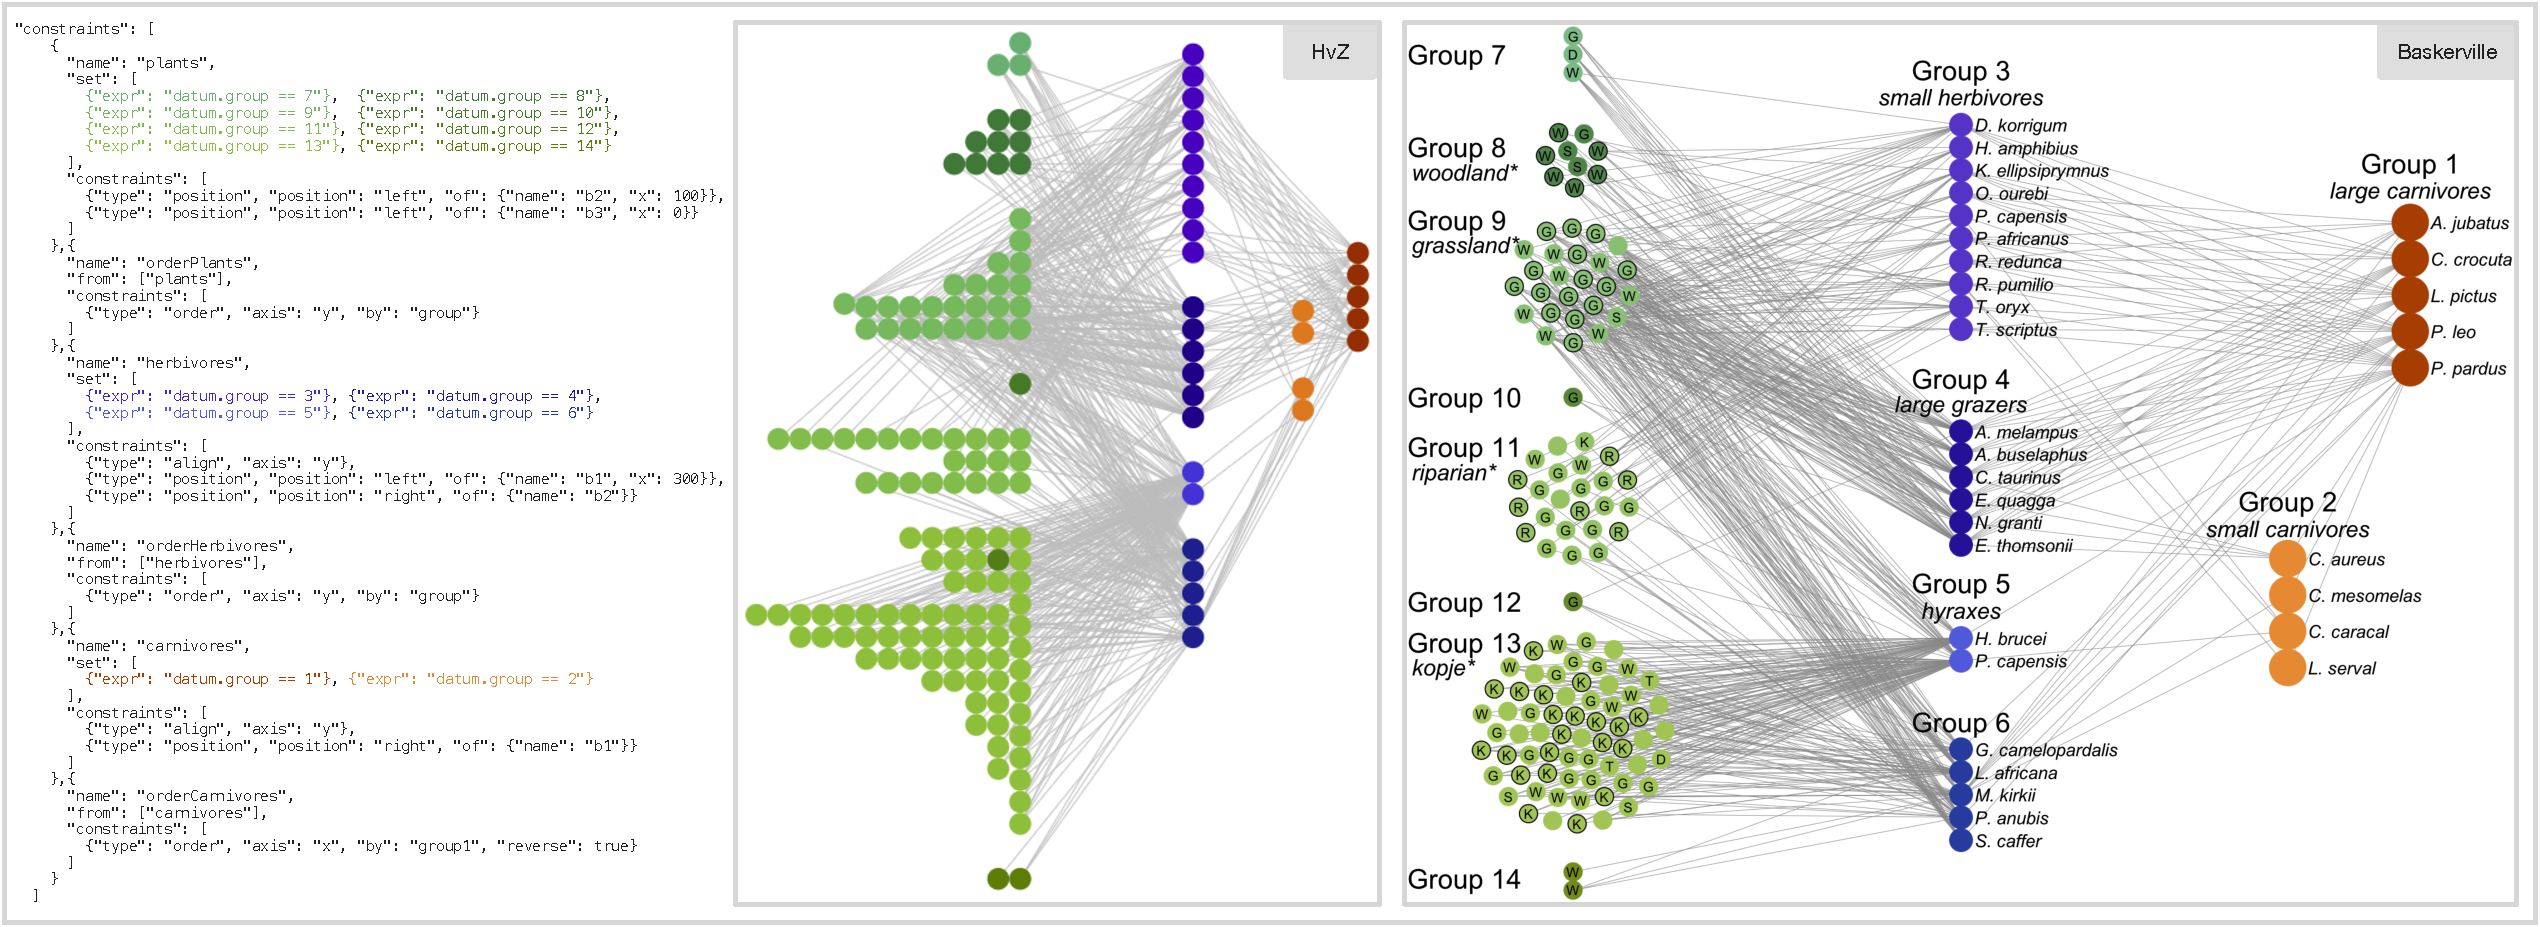
\includegraphics[width=\linewidth]{figures/serengeti-layout.pdf}
% 		\centering
% 	  \caption{\label{fig:teaser}}

% 	}
% }

\newcommand{\serengetiLayoutColumn}{
  \begin{figure}[t!]
    \centering
    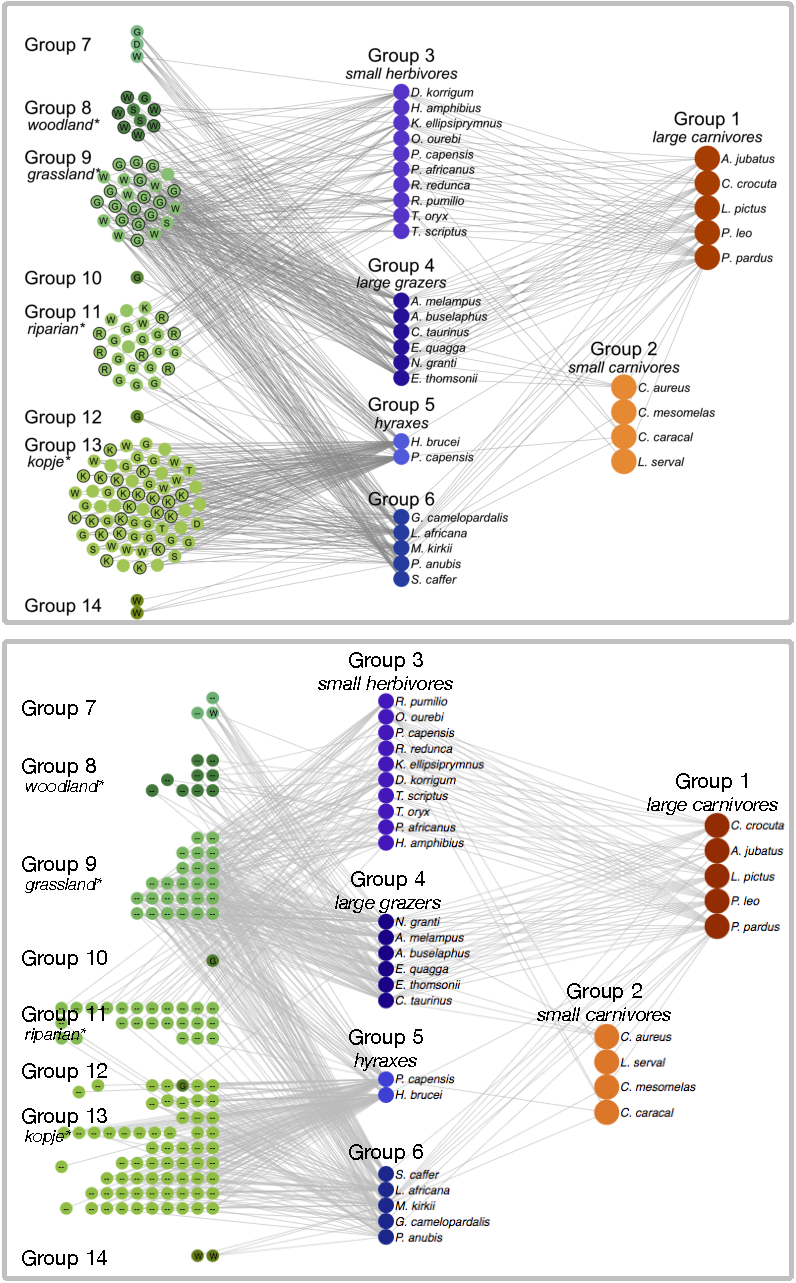
\includegraphics[width=0.81\columnwidth]{figures/serengeti-layout-column.pdf}
    {\caption{\label{fig:serengeti-layout}
    The layout for the Serengeti food web using our constraint language, as compared to Baskerville et al. \cite{baskerville2011spatial}.}}
    \vspace{-40px}
  \end{figure}
}

%%%%%%%%%%%%%%%%%%%%%%%%%%%%%%%%%%
%%%%%%%%%%%%% Design %%%%%%%%%%%%%
%%%%%%%%%%%%%%%%%%%%%%%%%%%%%%%%%%

\newcommand{\smallTreeExample}{
  \begin{figure}[t!]
    \centering
    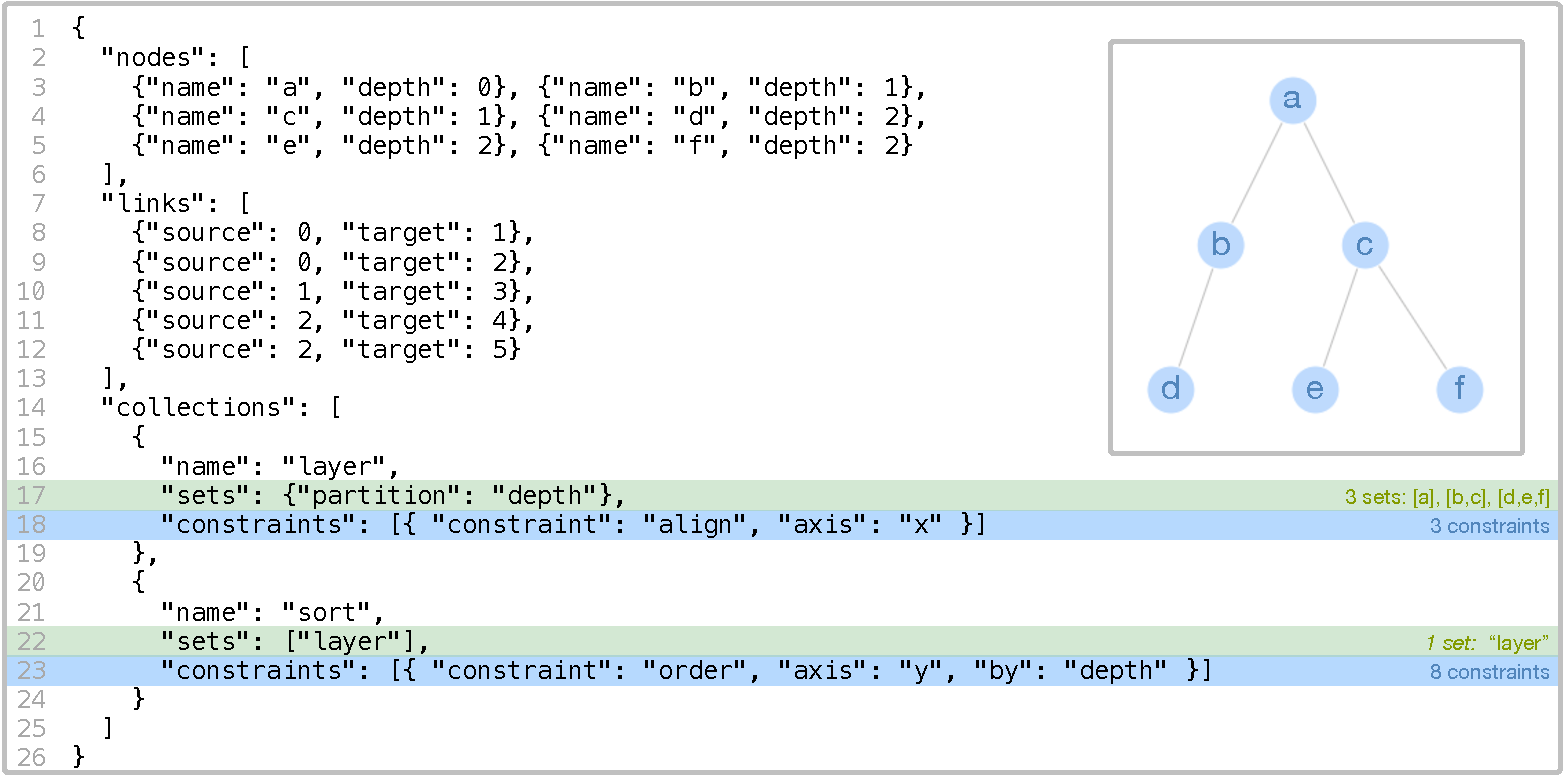
\includegraphics[width=\columnwidth]{figures/small-tree-example.pdf}
    {\caption{\label{fig:small-tree-example}
    The full \projectname\ specification for a small tree with six nodes. Nodes are split into sets based on their depth from the root \texttt{a}, and aligned. A new collection is formed containing the ``layer'' set and the layers are ordered by their depth to form the tree.
    }}
    \vspace{-20px}
  \end{figure}
}

\newcommand{\contradictionExample}{
  \begin{figure}[t!]
    \centering
    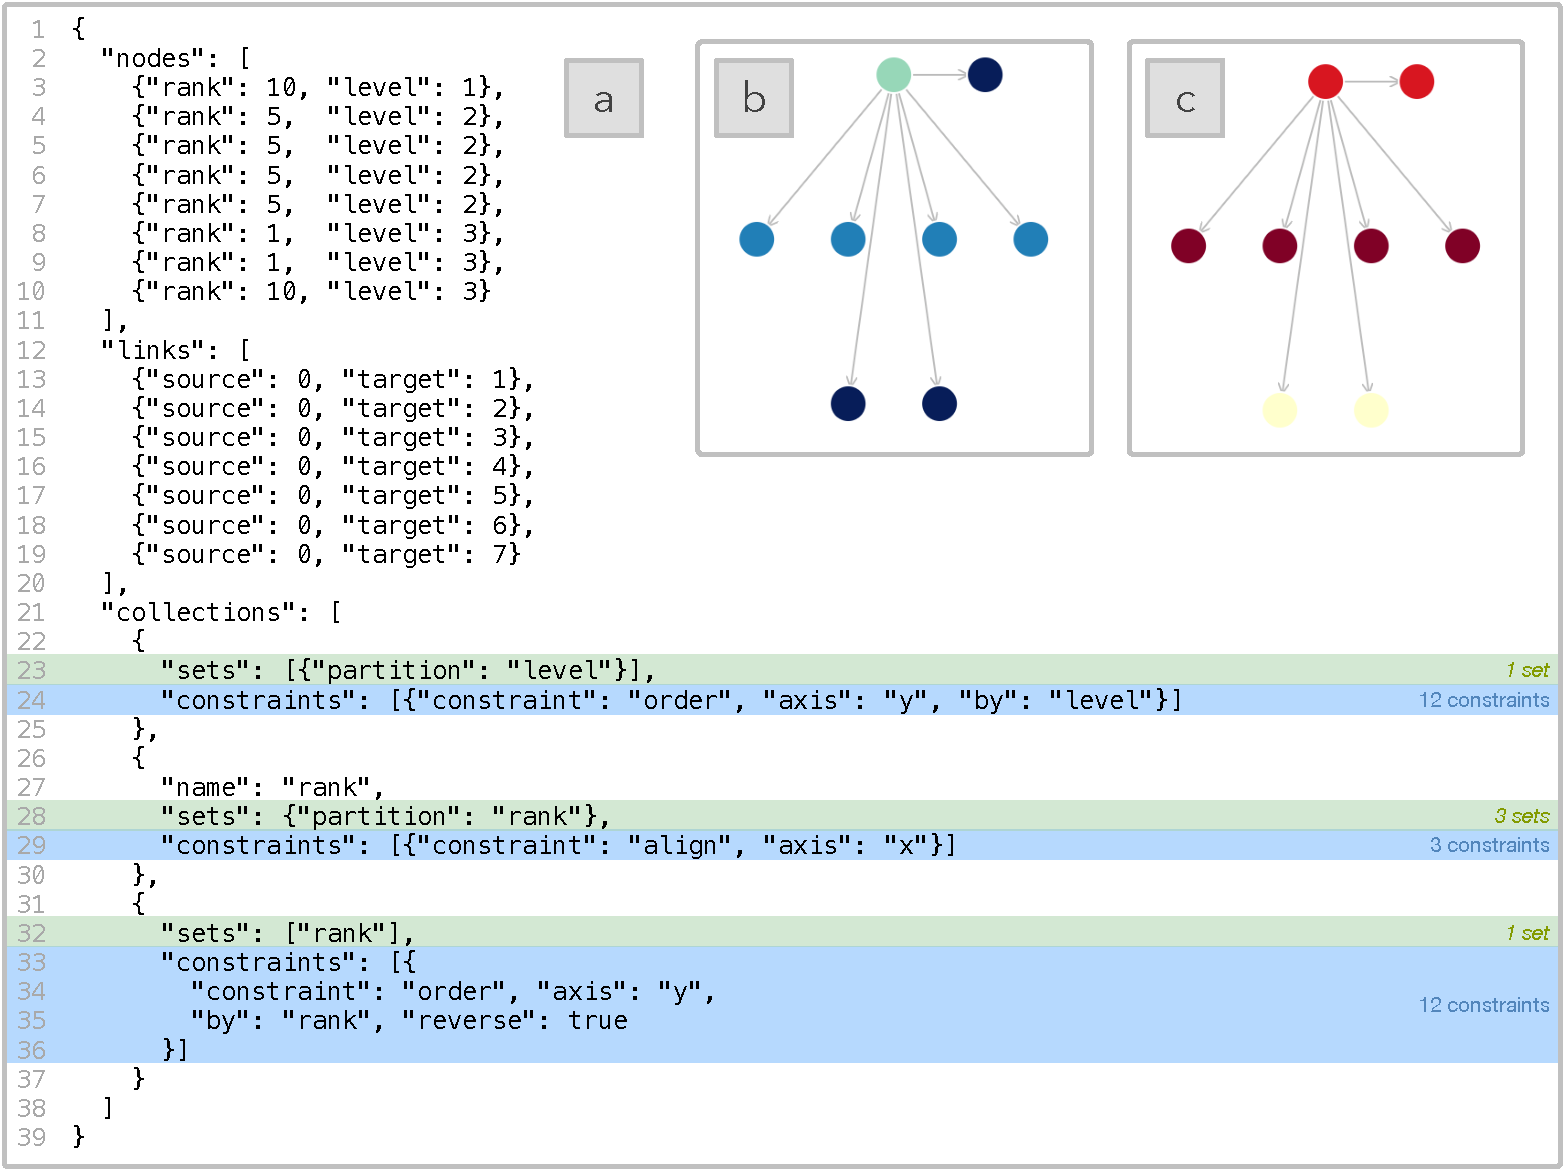
\includegraphics[width=\columnwidth]{figures/contradiction-example.pdf}
    {\caption{\label{fig:contradiction-example}
    (a) The full \projectname\ specification for a small graph with eight nodes. (b) Nodes are aligned based on their \texttt{rank}, and colored based on their \texttt{level}. Two constraints are applied to order the nodes, once by \texttt{level} and once by \texttt{rank}, which produces a contradiction. (c) Nodes are colored based on the amount of error for constraints that are invalid.
    }}
    \vspace{-20px}
  \end{figure}
}

%%%%%%%%%%%%%%%%%%%%%%%%%%%%%%%%%%
%%%%%%%%% Demonstration %%%%%%%%%%
%%%%%%%%%%%%%%%%%%%%%%%%%%%%%%%%%%

\newcommand{\krugerLayout}{
  \begin{figure}[t!]
    \centering
    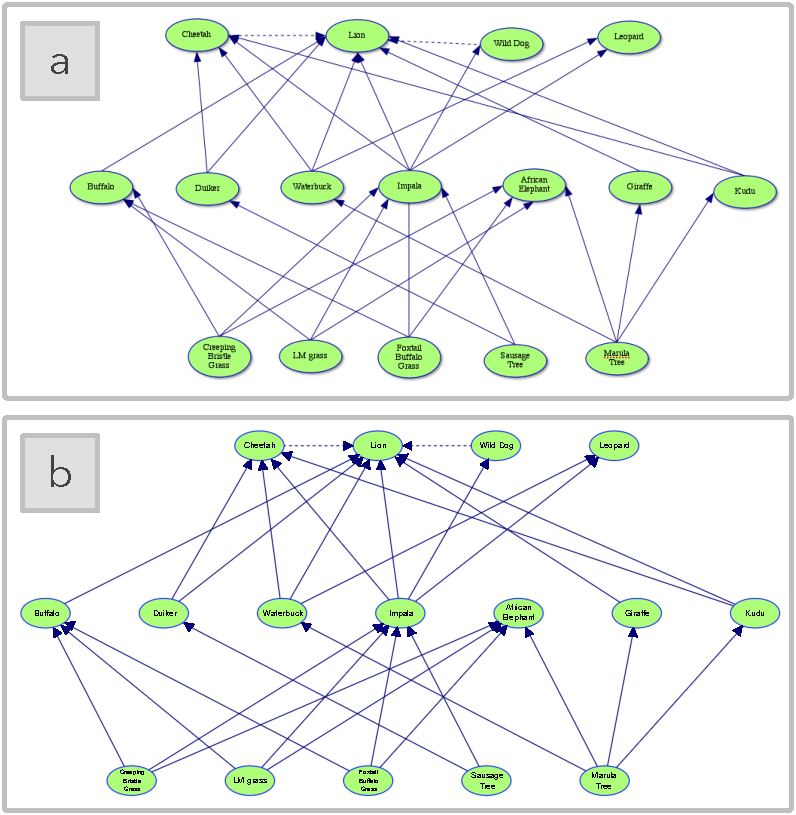
\includegraphics[width=0.81\columnwidth]{figures/kruger-layout.pdf}
    {\caption{\label{fig:kruger-layout}
    The layout for a small subset of the food web for Kruger National Park from (a) their website \orange{citation} as compared to (b) our layout using \projectname.}}
    \vspace{-20px}
  \end{figure}
}

\newcommand{\serengetiLayout}{
  \begin{figure*}[t]
    \centering
    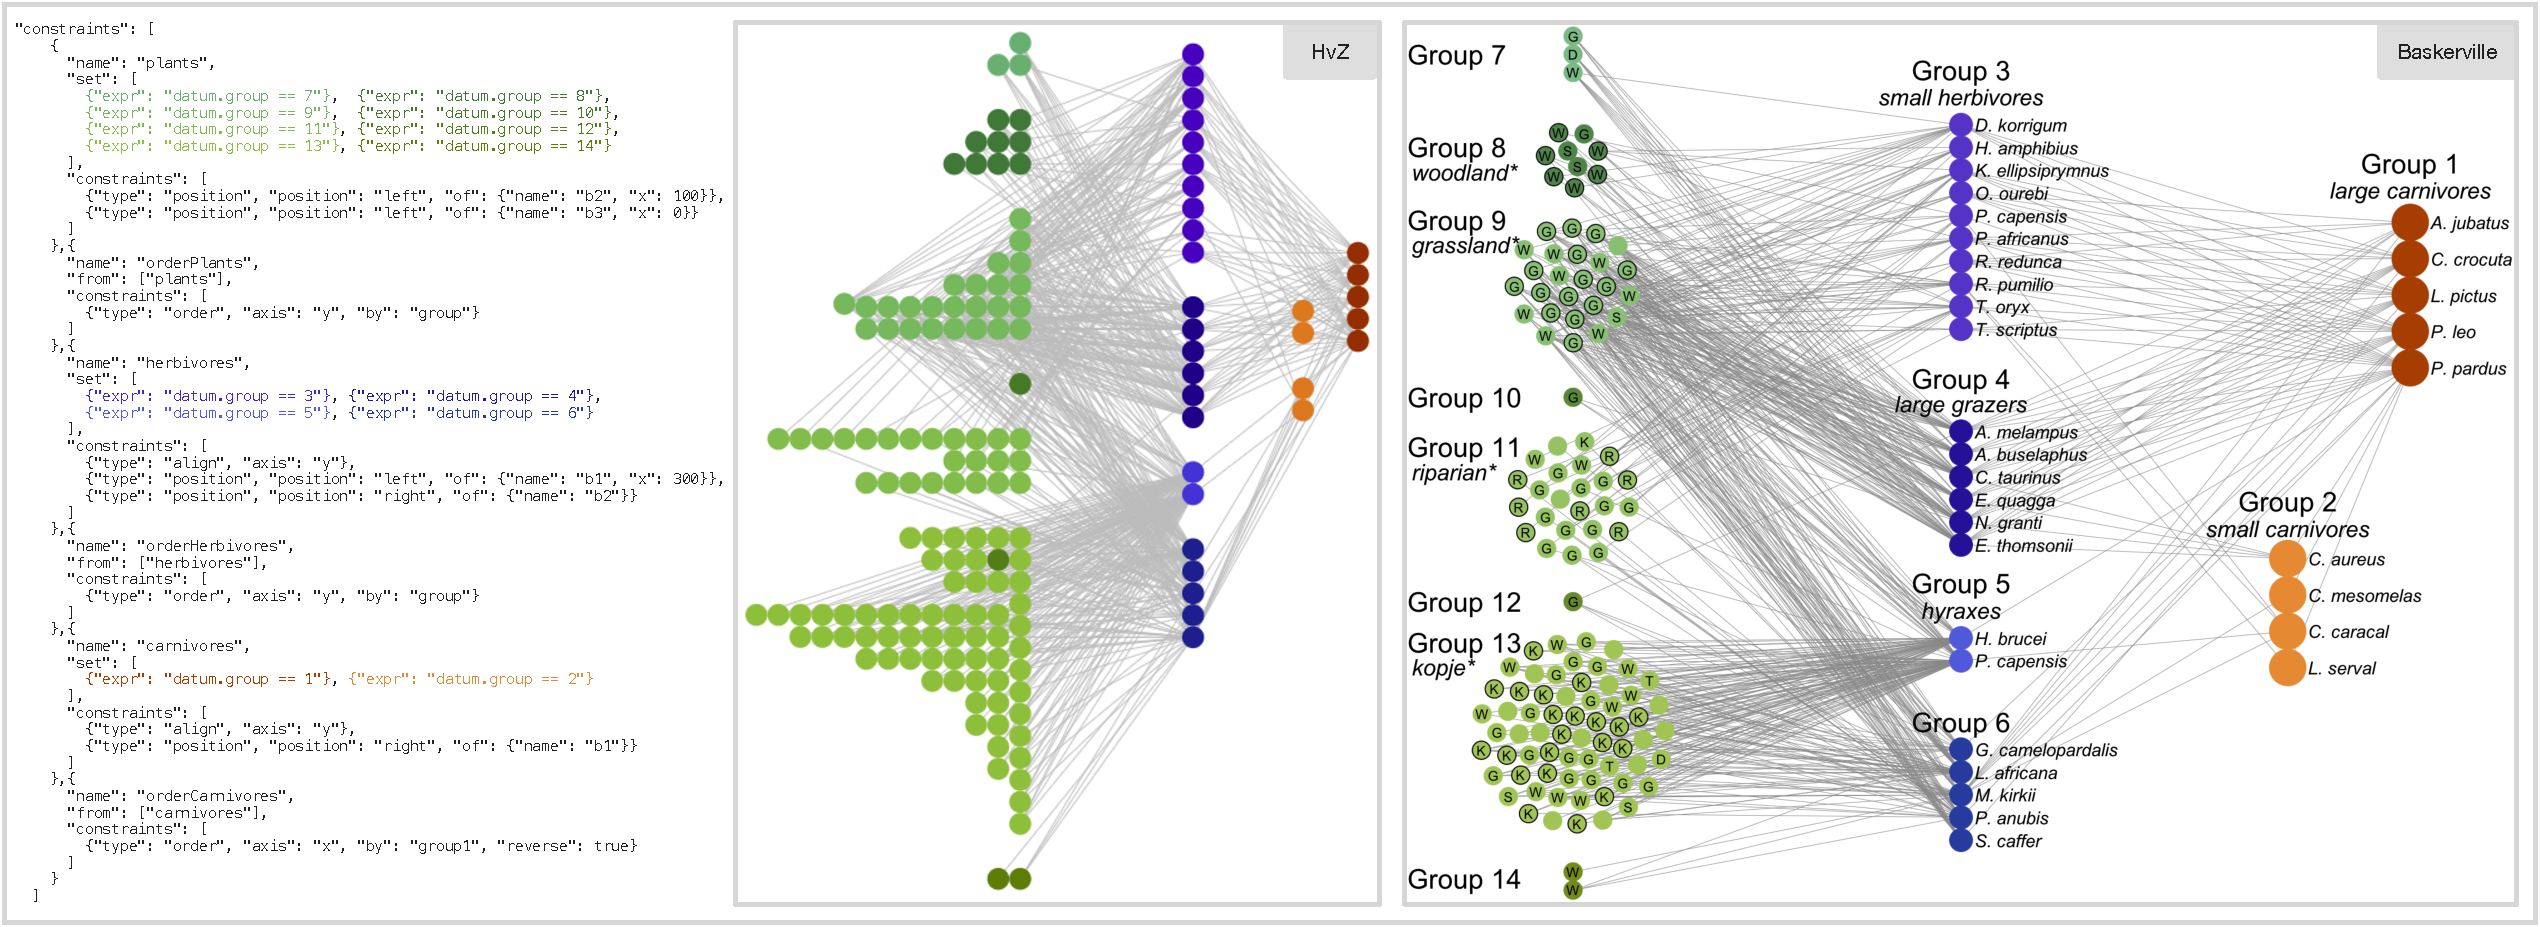
\includegraphics[width=\textwidth]{figures/serengeti-layout.pdf}
    \vspace{-20px}
    {\caption{\label{fig:serengeti-layout}
    The layout for the Serengeti food web using our constraint language, as compared to Baskerville et al. \cite{baskerville2011spatial}. \todo{retake photos on retina screen} \todo{label the two sides of the figure a/b}}}
  \end{figure*}
}

\newcommand{\serengetiSpec}{
  \begin{figure}[t]
    \centering
    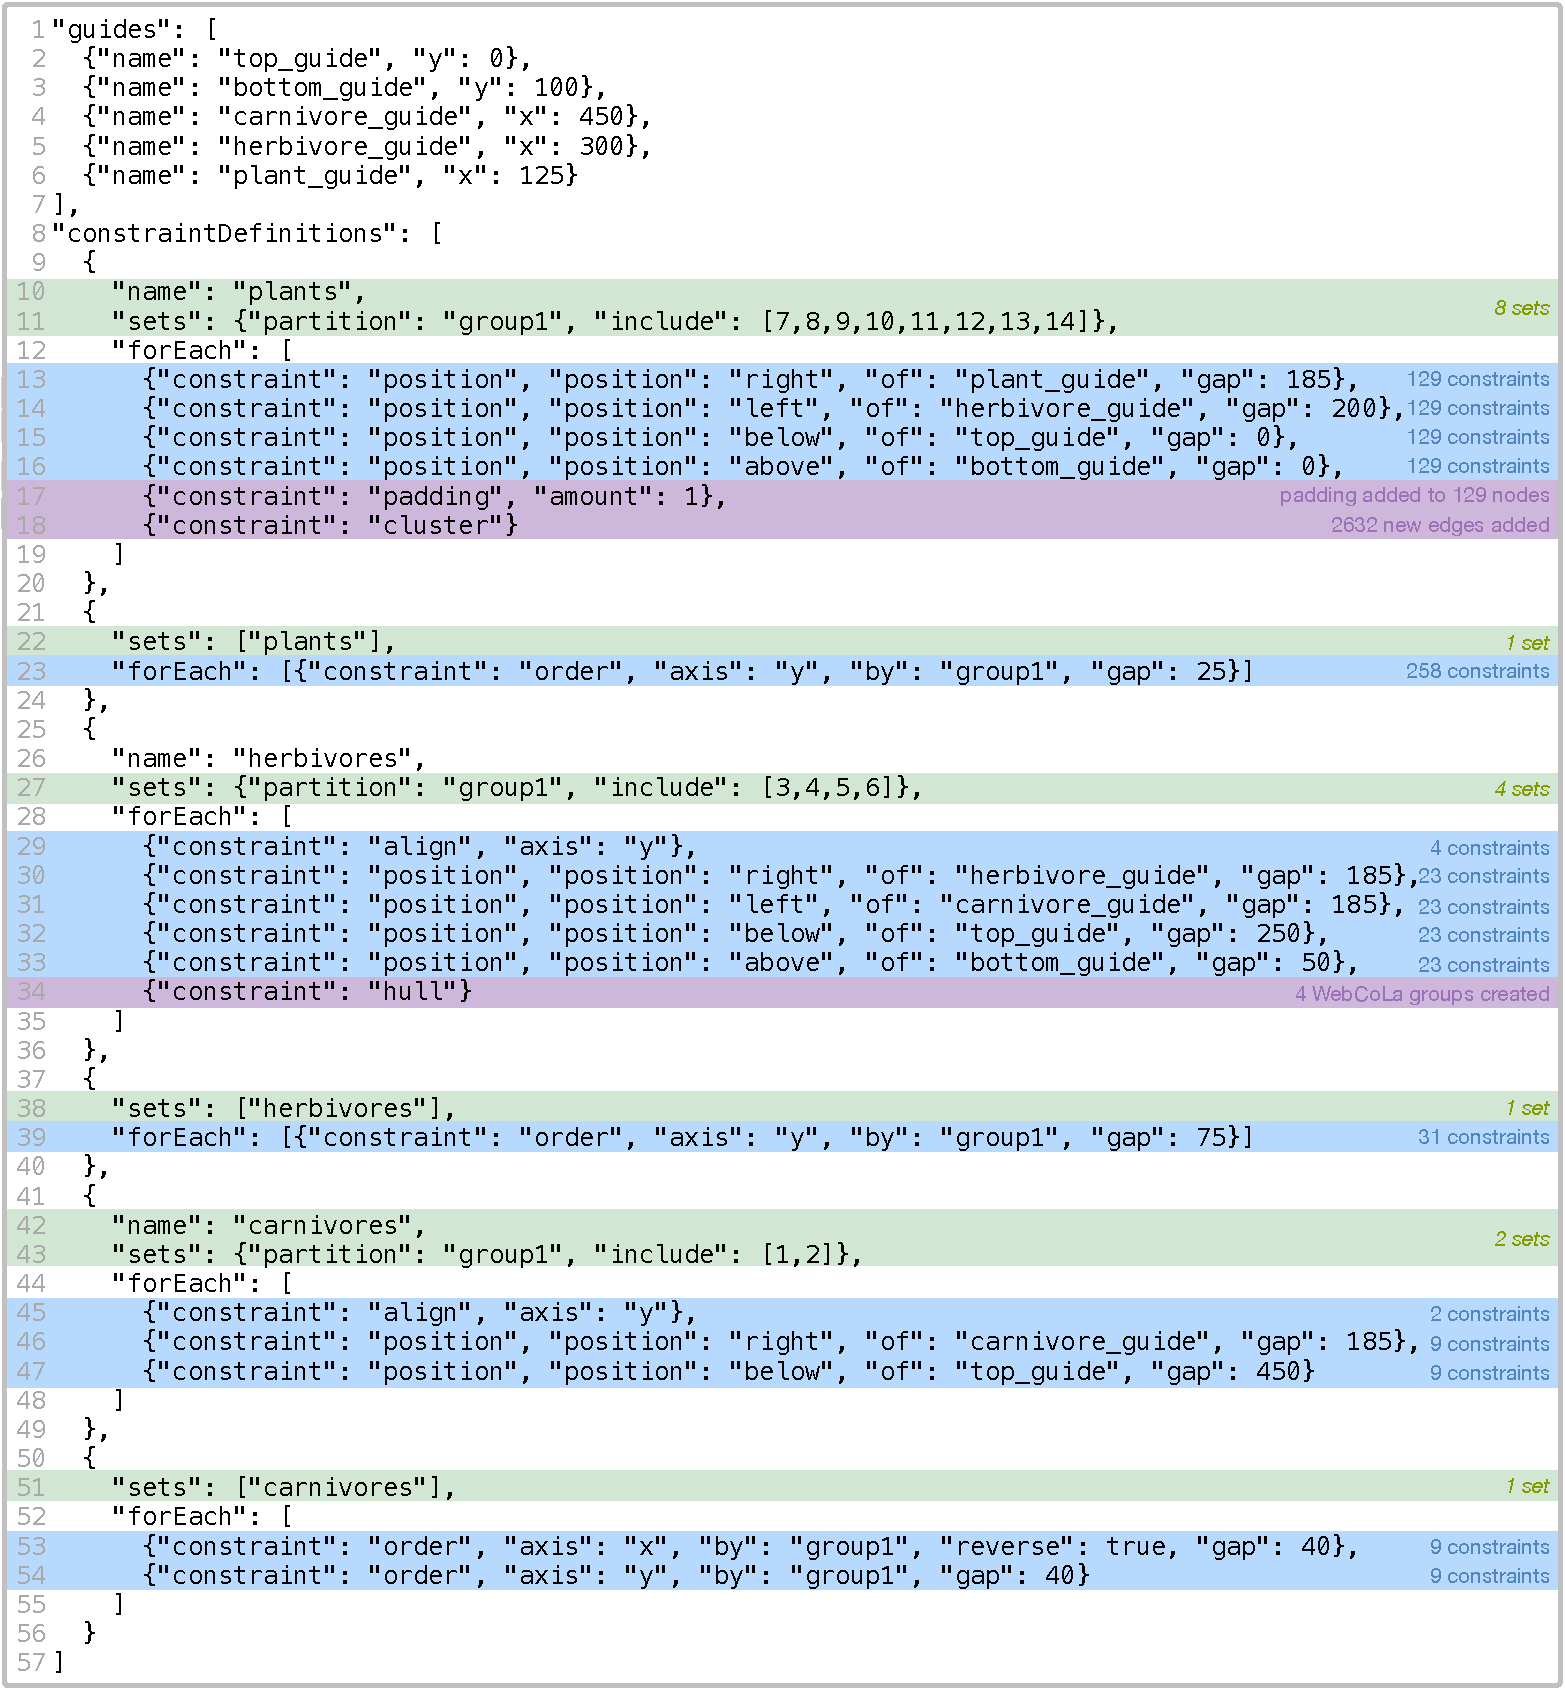
\includegraphics[width=\columnwidth]{figures/serengeti-spec.pdf}
    \vspace{-20px}
    {\caption{\label{fig:serengeti-spec}
    The \projectname~specification for the Serengeti food web shown in Figure~\ref{fig:serengeti-layout}. The code is annotated with the number of sets produced, the number of edges added, and the number of WebCoLa constraints generated for the final layout.}}
  \end{figure}
}

\newcommand{\syphilisLayout}{
  \begin{figure*}[t]
    \centering
    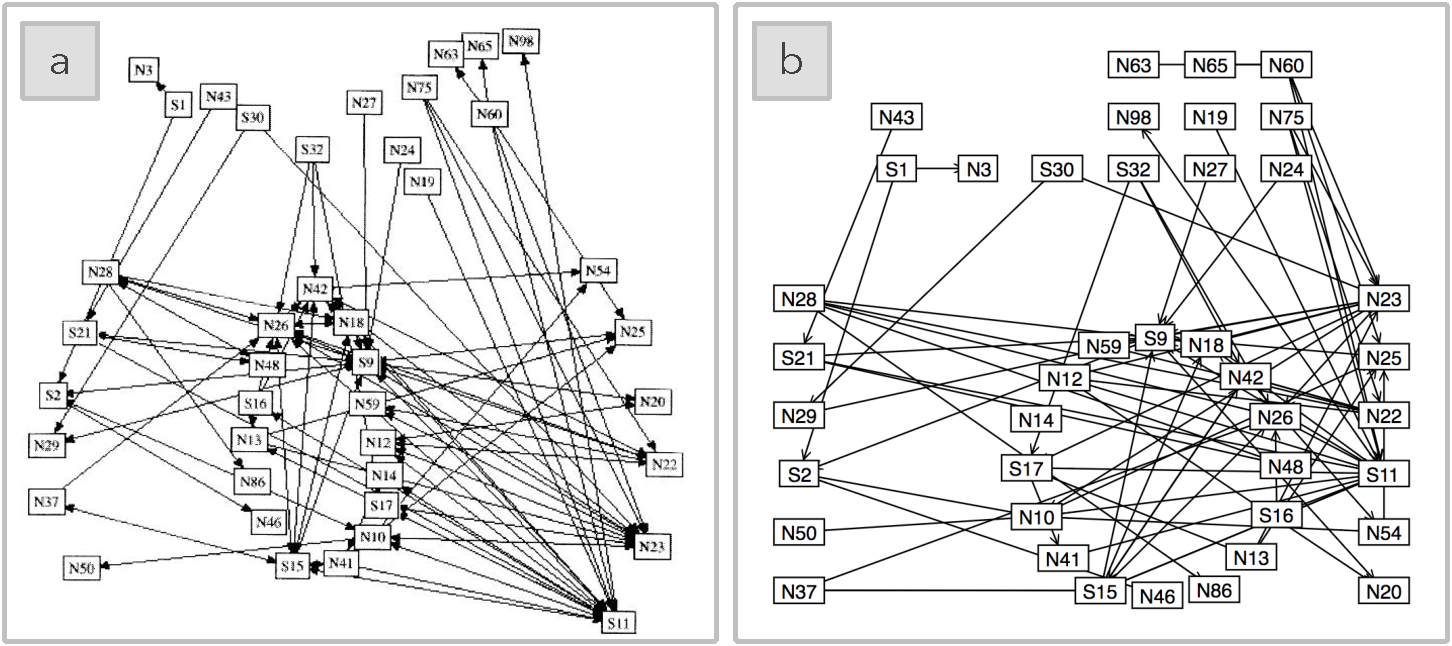
\includegraphics[width=\textwidth]{figures/syphilis-layout.pdf}
    \vspace{-20px}
    {\caption{\label{fig:syphilis-layout}
    The layout for the syphilis social network from (a) Rothenberg et al. \cite{rothenberg1998using} as compared to (b) the \projectname~layout. \todo{add some padding on the layout of the aligned men}}}
  \end{figure*}
}

\newcommand{\syphilisSpec}{
  \begin{figure}[t]
    \centering
    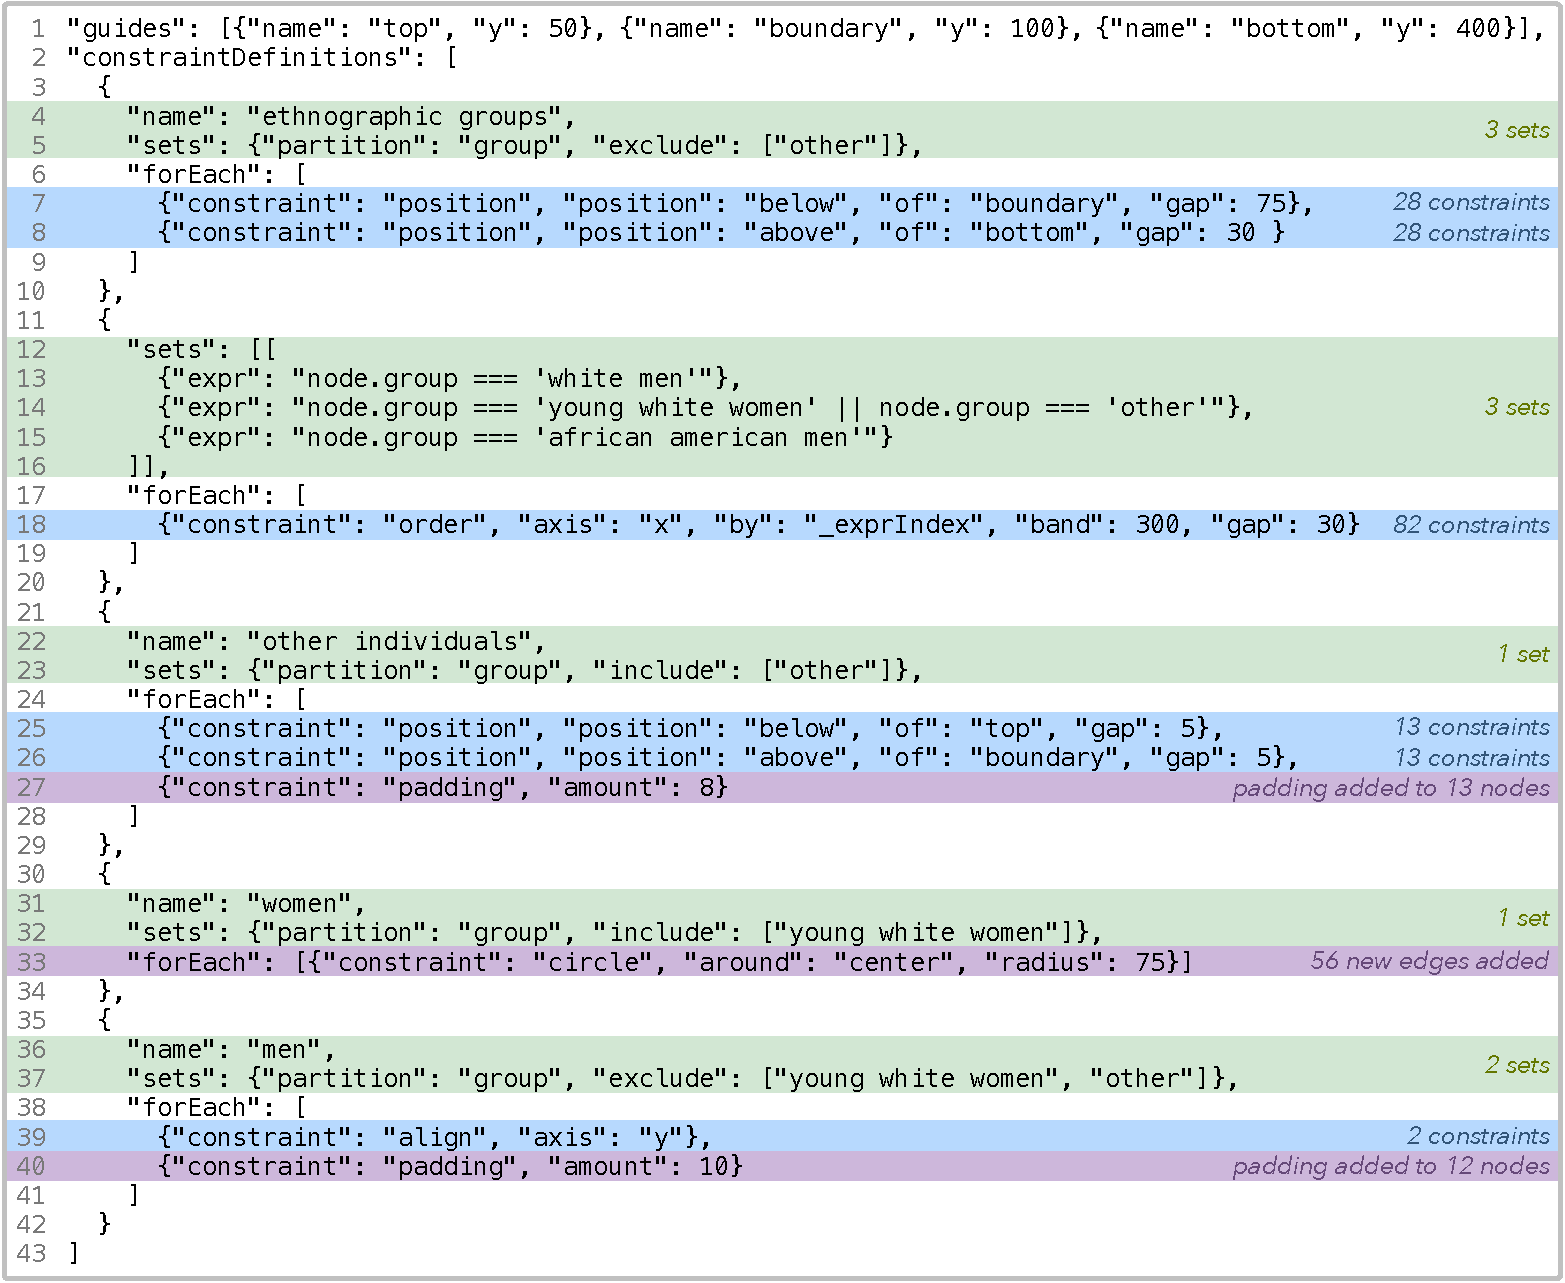
\includegraphics[width=\columnwidth]{figures/syphilis-spec.pdf}
    \vspace{-20px}
    {\caption{\label{fig:syphilis-spec}
    The \projectname~specification for the syphilis social network shown in Figure~\ref{fig:syphilis-layout}. The code is annotated with the number of sets produced, the number of edges added, and the number of WebCoLa constraints generated for the final layout.}}
  \end{figure}
}
%!TEX root = constraint-layout.tex
\section{Introduction}
Graph visualizations can effectively represent properties of the underlying data structure, such as the hierarchy or connectedness of the data within the graph layout. Such visualizations are common across domains including ecological networks \cite{hinke2004visualizing,harper2006dynamic,lavigne1996cod,baskerville2011spatial,yodzis1998local,cohen2003ecological,kearney2016blog,benson2016higher}, biological systems \cite{barsky2008cerebral,shannon2003cytoscape,gehlenborg2010visualization,saraiya2005visualizing,becker2001graph}, and \orange{third example from demonstration}, among many others. In order to emphasize relevant trends in the data, the graph layout may utilize domain specific details; for example, in an ecological network, nodes could be split by trophic level (plant, herbivore, or carnivore) (Figure~\ref{fig:serengeti-layout}). This customized layout can more effectively reveal the feeding relationships between trophic levels and the hierarchical structure.

% Provide a bit more info about what the layout tools are doing - an additional setnece/rewording
% Not sure about 'layout tool' - cerebral is a midpoint between algorithm and customized
\todo{extend discussion of what the layout tools are doing (and tools might not be the right word/framing, algorithm seems better)}
Many domain specific layout tools have been developed to address particular graphing needs \cite{barsky2008cerebral,shannon2003cytoscape,kearney2017d3,kearney2017ecopath}. However, when a layout tool does not exist for the domain or task of interest, users are required to either fit their data to one of the available tools or create a customized layout of their own. Creating such a customized layout often requires both domain and programming expertise. \todo{unclear who is collaborating at this point.}
% Unclear who is collaborating at this point; a visualization expert?
When collaboration is infeasible, domain experts may be required to invest large amounts of time into learning the skills necessary to program the customized layout themselves. Furthermore, these customized tools are hard to generalize beyond their domain; these tools are carefully crafted to meet the needs of a particular domain or task, which means that it can be hard for domain experts to share their new programming expertise with others. This barrier to creating highly customized, domain specific layouts means there is a gap between the analysis needs of some domains and the availability of tools to handle those needs.

\todo{talk about constraint based solutions and the shortcomings before introducing our approach}

% See more about constraint based solutions and what are the shortcomings
% talk about tedium of cosntraint side - and the constraint based approaches

\todo{Need to come up with a careful, descriptive definition of what I mean by customized layouts at some point in the intro}
To enable the design of customized domain specific layouts with minimal programming expertise, we present a high-level constraint language for graph layout. Users partition nodes into sets based on node or graph properties and apply layout constraints within or between these sets. This approach allows users to specify layout requirements at a high-level, while deferring the computation of the node-level constraints to the underlying system. These constraint specifications reduce programming effort while still enabling highly customized and generalizable graph layouts. We demonstrate the utility of this technique with an implementation of our constraint language that compiles our high-level constraints into inter-node constraints for WebCoLa~\cite{WebCoLa}, a JavaScript library for constraint based graph layout. To demonstrate the ease and extensibility of our language, we recreate a number of customized layouts with our WebCoLa implementation. We show that users can compactly specify complex graph layouts that resemble those produced by customized layout engines.
%!TEX root = human-constraint-layout.tex
\section{Related Work}
There are many areas of related work surrounding the visualization and layout of graphs, and domain specific graphs in particular. Graphs are a common type of data seen across a variety of domains including social networks \cite{scott1988social,travers1967small,granovetter1973strength,watts1998collective,freeman1978centrality}, biological systems \cite{barsky2008cerebral,shannon2003cytoscape,gehlenborg2010visualization,saraiya2005visualizing}, and ecological networks \cite{hinke2004visualizing,harper2006dynamic,lavigne1996cod,baskerville2011spatial,yodzis1998local,cohen2003ecological,kearney2016blog,benson2016higher}. In this section, we identify some common tools for graph layout and describe some tools that have been tailored for domain specific tasks.

\subsection{Graph Visualization}
Graph layout has been a long-standing area of research and there are a number of common layout techniques for visualizing graph data including tree layouts or force-directed layouts. Graphviz \cite{ellson2001graphviz} and Gephi \cite{bastian2009gephi} are two examples of visualization engines specific to graph layout. D3.js \cite{bostock:d3} is a JavaScript library that provides a number of built in layouts for graph data including force-directed and hierarchical layouts. WebCoLa \cite{WebCoLa} is a JavaScript library for constraint-based layout that can be used alongside D3 or Cytoscape~\cite{shannon2003cytoscape}.

In addition to these standard layout techniques, there is a large field of related work surrounding graph layout techniques that emphasize particular aesthetic or structural properties in the graph. HOLA \cite{kieffer2016hola} presents a layout engine to produce layouts similar to those produced by hand by identifying common aesthetic properties of the graph used in manual layouts and using the results to drive the design of a new layout algorithm. Kieffer et al. \cite{kieffer2013incremental} present a constraint-based layout for creating graphs with node and edge alignment, and demonstrate the feasibility of such a technique in an interactive system, Dunnart \cite{dwyer2008dunnart}.

While these are some examples of customized layouts, the customization reflects general properties of the graph as opposed to domain specific details. Our work focuses on providing a general language for supporting customized graph layouts with minimal programming expertise.

\subsection{Domain Specific Graph Visualization}
\smallTree
To address the domain specific needs for graph analysis, a number of tools have been developed to utilize domain specific information in the layout. Cerebral \cite{barsky2008cerebral} is a tool designed to visualize biological systems and support interactive exploration of different experimental conditions. Cytoscape \cite{shannon2003cytoscape} is a visualization system designed to explore biomolecular interaction networks and provides a framework for accepting customized plugins to extend the system. Becker and Rojas \cite{becker2001graph} provide a customized algorithm for visualizing metabolic pathways. Kearney has developed D3 \cite{kearney2017d3} and Ecopath \cite{kearney2017ecopath} plugins to aid in the visualization of food webs.

Each of these tools was designed with a particular domain in mind to address the needs of domain experts who were unable to find the necessary support within existing tools. Our work aims to reduce the barrier of creating these customized systems by providing a compact way to specify domain specific graph layouts.

%!TEX root = human-constraint-layout.tex
\section{High-Level, User-Defined Constraints}
\smallTree
In this section we describe our constraint language for high-level, user-defined constraints. This languages includes support for specifying sets of nodes over which to run the constraints and three types of constraints over the nodes: \emph{alignment}, \emph{order}, and \emph{position}. Figure \ref{fig:small-tree} shows a small example specification for a tree layout and the resulting six node tree. 

We refer to two types of constraints throughout this paper: \emph{high-level} constraints and \emph{layout} constrains. \emph{High-level} constraints identify sets over which node-specific \emph{layout} constraints are applied. Every \emph{high-level} constraint must include a \texttt{"name"} property and specify sets over which to apply the \emph{layout} constraints. However, \emph{layout} constraints for a \emph{high-level} constraint are optional; in cases where \emph{layout} constraints are not provided, the user may simply want to define sets of nodes to refer to later in her constraint specification.

\subsection{Specifying Sets}
\label{sec:sets}
Every high-level constraint must specify a group of sets over which the layout constraints are defined. There are two types of high-level constraints that can be specified: \emph{within set} constraints and \emph{between set} constraints. \emph{Within set} constraints describe constraints that are applied to all of the nodes within a given set whereas \emph{between set} constraints describe constraints that are between larger sets. We describe how to define each type of constraint and show examples of how these constraints are applied.

\subsubsection{Within Set Constraints}
The user specifies within set constraints with the \texttt{"set"} property as shown for \texttt{alignLayer} in Figure \ref{fig:small-tree}. There are two ways to specify sets for within set constraints: the user can either partition all the nodes into disjoint sets or the user can specify expressions to create specific sets of nodes.

The simplest set definition is to \texttt{"partition"} nodes into sets based on a property of the node. When generating the sets, the system extracts the property of the node to use as the key for the set. Using \texttt{"partition"}, nodes can only occur in one set specification for the given constraint.

There are two additional properties that users can apply to set partitioning: \texttt{"include"} and \texttt{"ignore"}. \texttt{"include"} allows the user to specify a property of the accepted node to \emph{include} in the set. This property must also be a node, for example the \texttt{"parent"} or \texttt{"firstchild"} of the node \green{add a figure that shows this}. \texttt{"ignore"} represents a list of keys to \emph{ignore} when creating the sets. This property can be useful for preventing nodes with specific properties from being included in the layout (e.g. the \texttt{layer} constraint of Figure \ref{fig:tlr4-layout}).

Alternatively, the user can specify a concrete list of sets to compute. In this representation, the user defines an expression that returns a boolean value of whether or not the node should be included in the set. The user may also specify an optional \texttt{"name"} property that is used by the debugging tools. Using this syntax, users may specify sets such that a node can appear in multiple sets. However, we currently throw an error when such a specification occurs. Future work is required to determine whether or not this behavior would be useful for complex layouts. The \texttt{"expr"} definition currently supports value comparisons (e.g. \texttt{==}, \texttt{<=}, \texttt{>}), and conjunctions (\texttt{\&\&}) and disjunctions(\texttt{||}) of value comparisons and boolean values. The user may use \texttt{datum.property} to refer to properties of the node.

Within set constraints define constraints that should be applied to all nodes in a set separate from nodes outside the set. In Figure~\ref{fig:small-tree}, the user partitions nodes into sets based on their depth and creates an \emph{alignment} constraint to align the nodes in each set along the x-axis.

\subsubsection{Between Set Constraints}
The user specifies between set constraints using the \texttt{"from"} property as shown by the \texttt{orderLayers} constraint in Figure~\ref{fig:small-tree}. The user specifies between set constraints as a list of previously named constraints. Between set constraints define constraints that should be applied between sets but not between nodes in a given set. In Figure~\ref{fig:small-tree}, the user selects all the sets defined by \texttt{alignLayer} and creates an \emph{order} constraint to sort the sets by their depth along the y-axis.

\subsection{Specifying Constraints}
Once the user has defined sets of nodes over which to apply the constraints, she may optionally define layout constraints for that specification. Every cosntraint must have a \texttt{"type"} property that defines the type of constraint. We support three types of layout constraints: \emph{alignment} (\texttt{"align"}), \emph{order} (\texttt{"order"}), and \emph{position} (\texttt{"position"}).

\subsubsection{Alignment Constraints}
Alignment constraints are the easiest constraint to specify in our constraint language and define using WebCoLa. Alignment constraints must have two properties, \texttt{"type"} and \texttt{"axis"}. The property \texttt{"axis"} can be defined as either \texttt{"x"} or \texttt{"y"}. Figure~\ref{fig:small-tree} shows an example of \emph{alignment} for the high-level constraint \texttt{alignLayer}.

\subsubsection{Order Constraints}
Order constraints have three required properties: \texttt{"type"}, \texttt{"axis"} (either \texttt{"x"} or \texttt{"y"}), and \texttt{"by"}. The property \texttt{"by"} defines the property with which to order the nodes. If the \texttt{"by"} property does not have an obvious ordering (e.g. numeric, alphabetical), the user may optionally define an \texttt{"order"} property that is an ordered list of the expected inputs to the ordering function. The user may also optionally define a \texttt{"reverse"} property to reverse the behavior of the ordering. Figure~\ref{fig:small-tree} shows an example of an \emph{order} constraint for the high-level constraint \texttt{orderLayers}, which forces the layers to be positioned along the y-axis based on their depth.

\subsubsection{Position Constraints}
Position constraints have three required properties: \texttt{"type"}, \texttt{"position"}, and \texttt{"of"}. The property \texttt{"position"} accepts the values \texttt{"right"}, \texttt{"left"}, \texttt{"above"}, or \texttt{"below"}. The \texttt{"of"} property can be defined as a node, for example the \texttt{"parent"} or \texttt{"firstchild"} of the current node, or as a temporary point. The temporary point definition can include any combination of the properties \texttt{"name"}, \texttt{"x"}, and \texttt{"y"}. If \texttt{"x"} or \texttt{"y"} is not defined, it is initialized to zero by default. Specifying a \texttt{"name"} property allows the new node to be reused in different parts of the specification. The temporary nodes are optionally visualized in the layout and can be used to modify the final layout by moving the nodes. An example of this behavior is shown in Figure \ref{fig:serengeti-iterations}b,c.

\subsection{Built-in Properties}
The constraint specification can use any properties of the nodes in the original graph. However, we also provide a number of built-in properties that can be defined over the nodes. These properties are automatically computed and added to the graph specification prior to computing the final WebCoLa constraints. These properties are only added to nodes if such a property does not already exist on the nodes.

\begin{description}
\item[\texttt{\_id}] The index of the node in the graph specification.
\item[\texttt{depth}] One more than the max depth of the node's parents. This property is only allowed if the graph contains only one root node and does not contain cycles.
\item[\texttt{parent}] The parent of the current node. This property is only allowed if the node has one parent or is defined as the parent with the smallest \texttt{"\_id"}.
\item[\texttt{firstchild}] The child node of the current node with the smallest \texttt{"\_id"}.
\item[\texttt{parents}] The list of nodes that have edges where the current node is the target.
\item[\texttt{children}] The list of nodes that have edges where the current node is the source.
\item[\texttt{neighbors}] The list of nodes that have edges connected to the current node. This property is the join of the \texttt{"parents"} and \texttt{"children"} properties.
\item[\texttt{degree}] The number of \texttt{"neighbors"}.
\end{description}

%!TEX root = constraint-layout.tex
\section{Implementation of \projectname~using WebCoLa}
We created an implementation of \projectname\ in which we generate node
specific constraints in WebCoLa~\cite{WebCoLa} based on our high-level
constraints. WebCoLa is an open-source JavaScript library for
creating high-quality, stable constraint layouts, and was therefore a
useful back end to demonstrate the utility of \projectname\ on a number of
examples (see Section \ref{sec:examples}). In this section, we discuss the
constraint generation process for producing WebCoLa constraints and the 
addition of built-in properties of the graph structure.

%%%%%%%%%%%%%%%%%%%%%%%%%%%%%%%%%%%%%%%%%%%%%%%%%%%%%%%%%%%%%%
\subsection{Generating WebCoLa Constraints}

\todo{Describe the constraint generation procedure for within and between
  sets as well as the number of constraints that each one generates.}

%%%%%%%%%%%%%%%%%%%%%%%%%%%%%%%%%%%%%%%%%%%%%%%%%%%%%%%%%%%%%%
\subsection{Built-In Properties of the Graph Structure}
In addition to defining constraints relative to properties arising from
the domain, it may also be important to define constraints on properties
of the graph structure. In our WebCoLa implementation, we support a 
number of built-in properties for the nodes that reflect the graph structure.
These properties are automatically computed and added to the graph 
specification when they are used in one of the \projectname\ constraints. 
These properties are only computed if such a property does not
already exist on the nodes and are subject to a number of expectations
regarding the graph input; for graphs that do not meet these expectations,
users are shown a warning and required to compute the properties
themselves.

\begin{description}
\item[\texttt{\_id}] The node index in the graph specification. This
  property is always computed regardless of whether or not it is used.
\item[\texttt{depth}] One more than the max depth of the node's
  parents. This property is only computed for graphs that contain only one
  root node and do not contain cycles. \todo{Is there a definition for
  graphs with multiple roots (or can we handle disconnected graphs)? Can
  the user specify the root in the specification?}
\item[\texttt{parent}] The parent of the current node. This property is
  only allowed if the node has one parent; otherwise, it is defined as the
  parent with the smallest \texttt{\_id}.
\item[\texttt{firstchild}] The child node of the current node with the smallest \texttt{\_id}.
\item[\texttt{incoming}] The list of nodes that have edges where the
  current node is the target (e.g., all parent nodes).
\item[\texttt{outgoing}] The list of nodes that have edges where the
  current node is the source (e.g., all child nodes).
\item[\texttt{neighbors}] The list of nodes that have edges connected to
  the current node. This property is the join of the \texttt{incoming} and
  \texttt{outgoing} properties.
\item[\texttt{degree}] The number of \texttt{neighbors}.
\end{description}

\todo{confirm all descriptions}

We selected these properties as common structural elements that could be
applicable to layout specifications. For example, the \texttt{depth}
property is useful for producing hierarchical tree layouts and the 
\texttt{incoming}, \texttt{outgoing}, and \texttt{neighbors} properties
reflect structure produced by the graph edges. There are many other
properties that could be useful for graph layouts that are not included 
here; this list could easily be extended in the future to include other
common properties. Furthermore, additional properties can always be
computed by the user and added to the graph prior to running the layout.
%!TEX root = human-constraint-layout.tex
\section{Usage Scenario}
%!TEX root = constraint-layout.tex
\section{Conclusion}
We present \projectname: a domain-specific language for specifying high-level
constraints for customized graph layout. \projectname enables concise 
specification of layouts by applying constraints to node sets
rather than individual nodes. These customized layouts can
be reapplied to different graphs that share domain-specific properties.
We implemented \projectname using the WebCoLa library~\cite{WebCoLa} and demonstrate the expressiveness
of \projectname on real-world examples from ecological networks,
biological systems, and social networks. \projectname specifications reduce the
number of constraints written by the user by one to two orders of magnitude,
while enabling flexible and reusable domain-specific layouts.

\section*{Acknowledgements}
%\todo{Write acknowledgements section}
\textsc{Removed from anonymized submission.}



%% Acknowledgments
\begin{acks}                            %% acks environment is optional
                                        %% contents suppressed with 'anonymous'
  %% Commands \grantsponsor{<sponsorID>}{<name>}{<url>} and
  %% \grantnum[<url>]{<sponsorID>}{<number>} should be used to
  %% acknowledge financial support and will be used by metadata
  %% extraction tools.
  % This material is based upon work supported by the
  % \grantsponsor{GS100000001}{National Science
  %   Foundation}{http://dx.doi.org/10.13039/100000001} under Grant
  % No.~\grantnum{GS100000001}{nnnnnnn} and Grant
  % No.~\grantnum{GS100000001}{mmmmmmm}.  Any opinions, findings, and
  % conclusions or recommendations expressed in this material are those
  % of the author and do not necessarily reflect the views of the
  % National Science Foundation.
\end{acks}


%% Bibliography
%\bibliography{bibfile}


%% Appendix
%\appendix
%\section{Appendix}

%Text of appendix \ldots

\end{document}
